\chapter{Implementing Path-Tracing}
\label{chapter implementation}

To maximize rendering efficiency, this projects implements path-tracing with parallelization on GPUs. This chapter begins with an introduction to GPU computing, and then discusses some of the most impactful performance optimizations employed by this project. These include careful structuring of GPU kernels, avoidance of performance degradation caused by polymorphism, and most importantly, usage of Bounding Volume Hierarchies to accelerate intersection detections.

\section{The CUDA Programming Model}

Originally built for real-time rendering, GPUs can handle a massive amount of geometries and pixels in parallel. The ability to do massively parallel computation motivated GPGPU (General-Purpose GPU) programming models, which became significantly useful for high performance computing. The software in this project is written using the CUDA programming model, developed by the NVIDIA Corporation.

CUDA employs the execution model known as SIMT (Single Instruction Multiple Threads). In this model, a large amount of threads can be spawned simultaneously, each running the same code on different data. CUDA threads are organized in groups of 32, known as \textit{warps}. Each thread must execute the same instructions as the others in the same warp, or remain idle. When the threads within a warp access the memory, the entire warp can be paused and swapped out, so that a different warp can execute before the memory access finishes. Using this mechanism, the GPU hides memory access latencies by allowing very fast context switching. As a result, each physical core in the GPU can simultaneously handle multiple logical threads.

As an example, the GPU used for development of this project is an NVIDIA GTX1060 Mobile, which contains 10 \textit{Streaming Multiprocessors}, each of which consists of 128 CUDA cores. Each streaming multiprocessor can have up to 2048 resident threads, giving a total of 20480 threads that can be simultaneously handled. Even though each GPU thread is not as fast as a CPU thread, the aggregated performance of the CUDA cores can still be many times faster than the CPU.

% \begin{figure}[H]
%     \centering
%     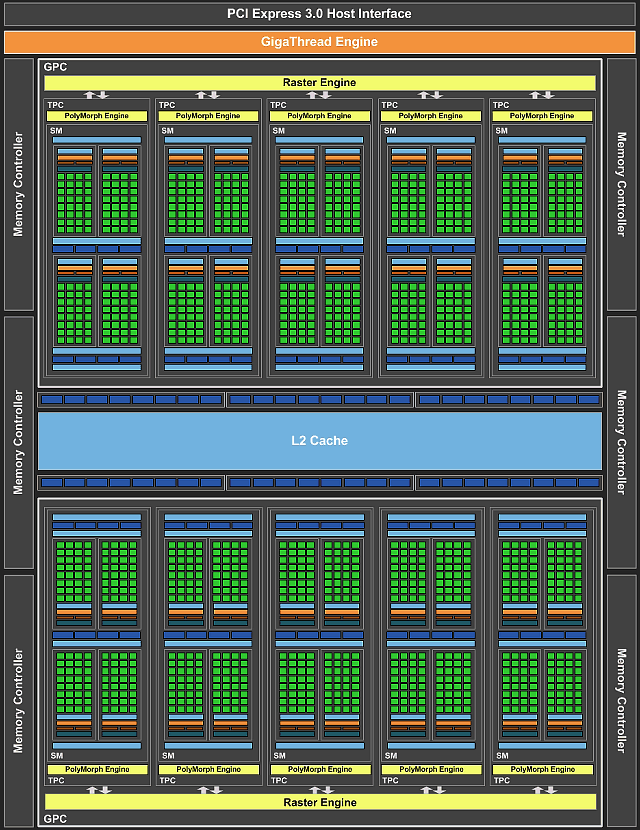
\includegraphics[width=11cm]{gp106}
%     \caption{Architecture of a GTX 1060 (GP106), showing its 10 streaming multiprocessors, each containing 128 CUDA cores. Image credit \cite{pascal}}
%     \label{figure GTX1060}
% \end{figure}
%https://images.nvidia.com/content/pdf/tesla/whitepaper/pascal-architecture-whitepaper.pdf



\section{Wavefront Path-Tracing}
In CUDA, a parallel GPU function that is invoked by the CPU is called a GPU \textit{kernel}. When implementing algorithm \ref{Path Tracing} on GPUs, the most straightforward method is to implement the loop body (lines 3 to 12) as a GPU kernel, and invoke it for all pixel samples in parallel. This pattern of programming, where the entire computation is embodied in a single GPU kernel, is called the \textit{Megakernel}\cite{megakernel} approach.

In contrast to megakernels, the \textit{Wavefront} programming pattern divides the computation into many small kernels, where intermediate results are explicitly stored in memory. The CPU invokes these kernels one after another. On GPUs, regions of code that use a large amount of registers or have a high control flow divergence can significantly hurt the parallelization of the entire kernel, and thus the wavefront pattern can effectively contain these regions of code into separate kernels, so that the performance of the other kernels remain unaffected. However, the wavefront pattern incurs additional overhead by requiring more CPU-GPU communication, and memory IOs.

The project carried out numerous experiments to find an optimal way of dividing the rendering work into wavefronts. In the end, the program implemented is structured as indicated by the following pseudo-code:

\begin{algorithm}[H]
    \label{algo wavefront Path Tracing}
    \SetKwProg{Fn}{Function}{:}{end}
    \ForEach{\upshape pixel sample \textbf{in a parallel kernel}}{
        generate the initial ray $r_0$ going out of the camera position $p_0$\;
    }
    \For{\upshape $n$ from 1 to $MaxDepth$}{
        \ForEach{\upshape previously generated ray $r$ \textbf{in a parallel kernel}}{
            Find $p_n$ by computing the intersection between $r$ and the scene\;
            \If{\upshape $p_n$ is on a light source}{
                Accumulate the radiance of the path $p_n\to p_{n-1}\to ... \to p_0$\;
            }
        }
        \ForEach{\upshape newly found $p_n$ \textbf{in a parallel kernel}}{
            Sample a point $p_{light}$ on a light source\;
            Test whether the ray $p_{light}\to p_n$ occluded by some geometry\;
        }
        \ForEach{\upshape unoccluded $p_{light}\to p_{n}$ \textbf{in a parallel kernel}}{
            Accumulate the radiance of the path $p_{light}\to p_n\to ... \to p_0$\;
        }
        \ForEach{\upshape $p_n$ \textbf{in a parallel kernel}}{
            Sample a direction $\omega_i$ from a distribution matching the BRDF at $p_n$\;
            Generate a new ray, originated at $p_n$ and travels in the direction of $\omega_i$\;
        }
    }
    \caption{Wavefront Path Tracing}
\end{algorithm}

~

It was found that compared to a naive Megakernel implementation, this wavefront implementation is almost twice as fast.

\section{Polymorphism}
\label{section polymorphism}
In GPU programming, a common source of performance degradation is dynamic-dispatch polymorphisms. On CPUs, dynamic-dispatch is easily implemented via virtual functions, but this can be costly for GPUs for two main reasons:
\begin{enumerate}
    \item In the GPU, each thread in a warp must execute the same instructions as the others, or remain in idle. Thus, when different threads are dynamically dispatched to different code regions, control flow divergences occur, and the GPU becomes under-utilized.
    
    \item Virtual functions make use of virtual tables and virtual pointers. During dynamic dispatch, the value of the program counter needs to fetched by reading the correct entry from the virtual table. This adds an additional level of indirection, which is costly on the GPU where memory IOs are more expensive.
    
\end{enumerate}
The need for polymorphism in path tracing mainly comes from two components. Firstly, the scene to be rendered is often defined from various different geometric primitives (triangles, spheres, disks, etc.), and each primitive requires its own intersection detection code. Secondly, each object in the scene is associated with a certain surface material, and each material requires its own BRDF implementation. This project handles the polymorphism for these two components in different strategies.

For geometric primitives, this project chooses to completely eliminate the need for any primitive other than triangles. Before rendering begins, this project uses a pre-processing phase, where a triangle mesh is generated to represent each non-triangle primitive. This slightly increases rendering cost, because often a few thousands of triangles are needed to give a good approximation for shapes such as spheres. However, this overhead is outweighed by the benefit of reduced control flow divergences and memory IOs.

Unfortunately, polymorphism for materials cannot be handled in this manner, and thus it is impossible to avoid polymorphism all together. This project implements polymorphism not by virtual functions, but by using a templated \texttt{variant} class\footnote{\url{https://en.cppreference.com/w/cpp/utility/variant}}, where all polymorphic types are included as type arguments. As a pseudo-code example, the following type declaration could be used to define a general material type that could in fact be plastic, metal, or glass:
\begin{lstlisting}[style=cppStyle]
using Material = std::variant<Plastic, Metal, Glass>;
\end{lstlisting}

Implementation wise, a \texttt{variant} class is realized by \textit{tagged union}s, which is in essence the same technique used to implement sum types in languages such as Haskell. Dynamic dispatch can be provided not via virtual functions, but by switching on an integer label attached to the object. This effectively avoids the extra memory operation incurred by dereferencing virtual pointers.

The usage \texttt{variant} solves problem 2, but problem 1 still remains because control flow divergence still exists whenever threads in the same warp process different materials. To solve this problem, this project employs the method of \cite{megakernel}, which sorts the material evaluation tasks before they're executed. More precisely, in algorithm \ref{algo wavefront Path Tracing}, before the kernel at line 9 is executed, this project inserts an extra phase where all tasks are sorted according to the material at their respective $p_n$. This step groups together threads that work on the same material, and there will only be a few warps that experience any divergences. Even though the sorting incurs a small extra cost, it was observed that it considerably improves the overall rendering performance.

%\newpage


\section{Bounding Volume Hierarchy}
In path-tracing, the most expensive step is almost always ray-scene intersection detection. This is very frequent operation, appearing in line 5 and 8 of algorithm \ref{algo wavefront Path Tracing}. Thus, any performance gain in the intersection detection routine could prove to be significantly beneficial to the entire rendering procedure. 

In a naive implementation, intersection detection would be performed by iterating through all geometries, and testing for intersection against each. With $N$ being the amount of geometric primitives in the scenes, this is an $O(N)$ algorithm. Since $N$ is often in the order of millions, this linear time algorithm is unacceptably slow. For this reason, this projects implements a data structure known as Bounding Volume Hierarchy (BVH), which reduces the complexity down to $O(\log N)$.

The idea of BVH is to partition the geometric primitives into a hierarchy of disjoint sets. The sets are organized into a binary tree, so that the root node is the set containing all primitives, and the leaves are singleton sets. Each interior node $n$ has two disjoint children sets, and the union of the children sets is equal to $n$ itself. In BVH, each set of primitives is represented by an Axis-Aligned Bounding Box (AABB), which is a box where each edge is parallel to a coordinate axis. Each AABB represents the set of all primitives that are completely enclosed by the box. The following image shows an example 2D BVH:

\begin{figure}[H]
    
\centering

\tikzset{every picture/.style={line width=0.75pt}} %set default line width to 0.75pt        

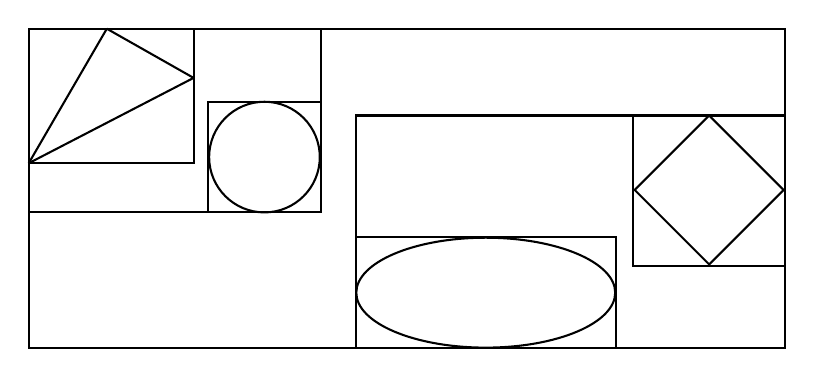
\begin{tikzpicture}[x=0.75pt,y=0.75pt,yscale=-1,xscale=1]
%uncomment if require: \path (0,300); %set diagram left start at 0, and has height of 300

%Shape: Rectangle [id:dp08780760692685319] 
\draw   (56,125) -- (420.44,125) -- (420.44,279) -- (56,279) -- cycle ;
%Shape: Rectangle [id:dp019517612425453468] 
\draw   (56,125) -- (196.76,125) -- (196.76,213.5) -- (56,213.5) -- cycle ;
%Shape: Rectangle [id:dp38178644543359463] 
\draw   (213.48,166.81) -- (420.44,166.81) -- (420.44,279) -- (213.48,279) -- cycle ;
%Shape: Rectangle [id:dp1975350888977112] 
\draw   (56,125) -- (135.44,125) -- (135.44,189.81) -- (56,189.81) -- cycle ;
%Shape: Ellipse [id:dp9801060884620203] 
\draw   (142.93,186.84) .. controls (142.93,172.12) and (154.86,160.19) .. (169.58,160.19) .. controls (184.3,160.19) and (196.24,172.12) .. (196.24,186.84) .. controls (196.24,201.56) and (184.3,213.5) .. (169.58,213.5) .. controls (154.86,213.5) and (142.93,201.56) .. (142.93,186.84) -- cycle ;
%Shape: Rectangle [id:dp6016074200382464] 
\draw   (142.41,160.19) -- (196.76,160.19) -- (196.76,213.5) -- (142.41,213.5) -- cycle ;
%Shape: Ellipse [id:dp7626275411333683] 
\draw   (213.83,252.17) .. controls (213.83,237.55) and (241.76,225.69) .. (276.2,225.69) .. controls (310.64,225.69) and (338.57,237.55) .. (338.57,252.17) .. controls (338.57,266.8) and (310.64,278.65) .. (276.2,278.65) .. controls (241.76,278.65) and (213.83,266.8) .. (213.83,252.17) -- cycle ;
%Shape: Rectangle [id:dp22500799968373997] 
\draw   (213.48,225.34) -- (338.91,225.34) -- (338.91,279) -- (213.48,279) -- cycle ;
%Shape: Rectangle [id:dp22604103897488237] 
\draw   (347.28,166.81) -- (420.44,166.81) -- (420.44,239.28) -- (347.28,239.28) -- cycle ;
%Straight Lines [id:da25863657063944623] 
\draw    (93.63,125) -- (56,189.81) ;
%Straight Lines [id:da9449132853969702] 
\draw    (93.63,125) -- (135.44,148.69) ;
%Straight Lines [id:da7107974477103463] 
\draw    (135.44,148.69) -- (56,189.81) ;
%Shape: Diamond [id:dp8408879189498177] 
\draw   (383.86,166.81) -- (419.75,202.7) -- (383.86,238.58) -- (347.97,202.7) -- cycle ;




\end{tikzpicture}

\end{figure}

In this example, there are 4 primitives, each occupying an AABB as a leaf node. One AABB groups together the triangle and the circle, and another groups the ellipse and the rombus. These two AABBs are then grouped together by the root AABB.


\subsection{BVH Traversal}
In a BVH, if one AABB doesn't intersect the ray, all descendent boxes can be pruned from the search. This motivates the following algorithm, which finds the first intersection point between a ray and a BVH node by traversing recursively:

\begin{algorithm}[H]
    \label{algo bvh traversal recursive}
    \SetKwProg{Fn}{Function}{:}{end}
    \Fn{\upshape \texttt{FindFirstIntersection}($node$, $ray$)}{
        \If{\upshape $node$ is a leaf node}{
            \uIf{\upshape $ray$ intersects with the geometry of $node$}{
                \Return{\upshape the intersection between $ray$ and this geometry}\;
            }
            \Else{
                \Return{\upshape ``No Intersections"}\; 
            }
        }
        \If{\upshape $ray$ does not intersect the AABB of $node$}{
            \Return{\upshape ``No Intersections"}\; 
        }
        Recursively, call \texttt{FindFirstIntersection}($node.leftChild$, $ray$) and \texttt{FindFirstIntersection}($node.rightChild$, $ray$)\;
        \uIf{\upshape both children do not intersect $ray$}{
            \Return{\upshape ``No Intersections"}\; 
        }
        \Else{
            \Return{\upshape the shortest intersection with one of the children nodes}\;
        }
    }
    \caption{Recursive BVH Traversal}
\end{algorithm} 

~

Unfortunately, this recursive traversal is unsuitable for implementation on GPUs. Firstly, GPUs have very restrictive recursion depth limits (for CUDA, this is 24), and thus might fail to complete the traversal. Secondly, due to the massive amount of parallel threads, maintaining a recursion stack for each thread is significantly costly in terms of memory and register usage. For these reasons, this projects explicitly maintains a stack of nodes to be traversed, and operates on this stack iteratively.

In addition to eliminating recursion, this project also makes two important observations that lead to a fruitful optimization. Firstly, the project notices that if it is known that a node can only produce intersections further than the current shortest intersection found, then it is useless to push it onto the stack. Secondly, the project notices that the intersection distance between the ray and an AABB is a lower-bound of the shortest intersection distance between the ray and any geometry in the AABB. Motivated by these observations, this project keeps track of the distance of the shortest intersection found, and then makes the following optimizations:
\begin{itemize}
    \item If a child node intersects the ray, but the ray-AABB intersection distance is further than the shortest intersection, then the node is discarded, because it cannot produce a shorter intersection.
    \item If both children nodes intersect the ray and are not discarded, then the node with the shorter intersection distance should be traversed first, because it has a higher chance of finding a better intersection.
\end{itemize}
Through experimentation, this project found that these techniques roughly double the efficiency of BVH traversal. The following pseudo-code summarizes the BVH traversal routine that this project implements:

\begin{algorithm}[H]
    \label{algo bvh traversal}
    \SetKwProg{Fn}{Function}{:}{end}
    \Fn{\upshape \texttt{FindFirstIntersection}($root$, $ray$)}{
        Create a stack $S$, with $root$ being the only element\;
        Let $minDistance := \infty$\;
        \While{\upshape $S$ is non-empty}{
            Pop a node $n$ from the stack\;
            \If{\upshape $n$ is a leaf node}{
                \uIf{\upshape $ray$ intersects with the geometry of $node$}{
                    Update $minDistance$ if this intersection is shorter than $minDistance$\;
                }
            }
            Compute $leftMinDistance$ as the minimum intersection distance between the left child AABB of $n$ with the ray\;
            Compute $rightMinDistance$ as the minimum intersection distance between the right child AABB of $n$ with the ray\;
            \If{\upshape exactly one child has intersection shorter than $minDistance$}{
                Push that child onto the stack\;
            }
            \If{\upshape both children have intersections shorter than $minDistance$}{
                Push the further child onto the stack\;
                Push the shorter child onto the stack\;
            }
        }
        \Return{\upshape the shortest intersection found}\;

    }
    \caption{Recursive BVH Traversal}
\end{algorithm} 

\subsection{BVH Quality Measure}

BVHs differ in quality, and these differences have a hugely impact on performance. Firstly, a BVH is binary tree, so the balance of the tree is related to the cost of the traversal. More importantly, notice that in algorithm \ref{algo bvh traversal}, it's possible that a ray $r$ intersects with both children of a node $n$, and thus both subtrees need to be traversed. A ``good'' BVH must reduce the likelihood of this type of situation. 

To formally quantify the quality of BVHs, this project employs the Surface Area Heuristic (SAH), first introduced in \cite{goldsmith1987automatic}. The SAH heuristic estimates the expected cost of a single BVH traversal for a random ray, and it is compute by
\begin{align*}
    C_i \sum_{n\in I} \Pr(\mathcal{X}_n) + C_l \sum_{n\in L} \Pr(\mathcal{X}_n)
\end{align*}
where $I$ is the set of interior nodes, $L$ the set of leaves, $C_i$ the cost for intersection testing a single interior node, $C_l$ the cost for intersecting testing a leaf node, and $\mathcal{X}_n$ the event that a random ray intersects the node $n$. SAH uses the observation that, for a convex shape $S_1$ enclosed within another convex shape $S_2$, the conditional probability $\Pr(\mathcal{X}_{S_1} | \mathcal{X}_{S_2})$ is exactly equal to $\frac{A(S_1)}{A(S_2)}$, where $A$ is the function that computes surface area. Thus, the SAH heuristic becomes
\begin{align*}
    C_i \sum_{n\in I} \frac{A(n)}{A(root)} + C_l \sum_{n\in L} \frac{A(n)}{A(root)}
\end{align*}

Given a collection of primitives, finding the optimal BVH tree according to the SAH heuristic is an NP-hard problem \cite{bvh_optimize}. This is not entirely surprising, considering the fact given any node with $N$ geometries, there are $2^N-2$ ways of constructing the two children nodes. However, not all hope is lost if the goal is to construct a BVH that's not necessarily optimal, but still reasonably good. This project implements a two-step system to approach high-quality BVH construction:

\begin{enumerate}
    \item Firstly, construct a BVH using a naive heuristic: at each node, split the AABB at the mid-point of a coordinate axis, thereby dividing the geometries into two groups. This is known as a Linear BVH, which can be constructed efficiently on GPUs using the method of \cite{bvh_build}, but the tree created is of poor quality.
    \item Secondly, optimize the previously created BVH tree, using the method of \cite{bvh_optimize}. This step repeatedly solves the NP-hard optimization problem for very small \textit{treelets}, which can still significantly improve the quality of the entire tree.
\end{enumerate}
This two-step approach is similar to the BVH construction routine of NVIDIA's Optix library. Details for the two steps are described below.

\subsection{Linear BVH Construction}
In Linear BVH, the AABB of each node is split at the mid-point of a coordinate axis, dividing the geometries into two groups. In three dimensions, the X, Y, and Z axises are used for splitting in a round-robin fashion, as the depth of the tree increases. A naive implementation of this splitting method would start at the root of the tree, and recursively divide each node using this heuristic. Unsurprisingly, this recursive algorithm parallelizes poorly. This motivates this project to employ a more sophisticated method described at \cite{bvh_build}, which uses a spatial encoding called \textit{morton code} and a data structure known as \textit{binary radix tree}.

The algorithm begins by taking the centroid of each geometric primitive. The algorithm scales and rounds each component of the centroid, so that it is represented by a 21-bit integer. Then, using the integer tuple $(x,y,z)$ which represents the position of the centroid, the algorithm computes its \textit{morton code}, which is a 63-bit integer defined as
$$ M=x_0~y_0~z_0~x_1~y_1~z_1~...~x_{20}~y_{20}~z_{20} $$
where $x_i$ is the $i$th bit of the $x$-coordinate, and the same for $y_i$ and $z_i$. As an example, the image below illustrates a two dimensional 6-bit morton code. For each pair of $(x,y)$ coordinate, its morton code $M$ is the index of the point along the zig-zag curve which begins at the lower left corner.
\begin{figure}[H]
    \centering
    


\tikzset{every picture/.style={line width=0.75pt}} %set default line width to 0.75pt        

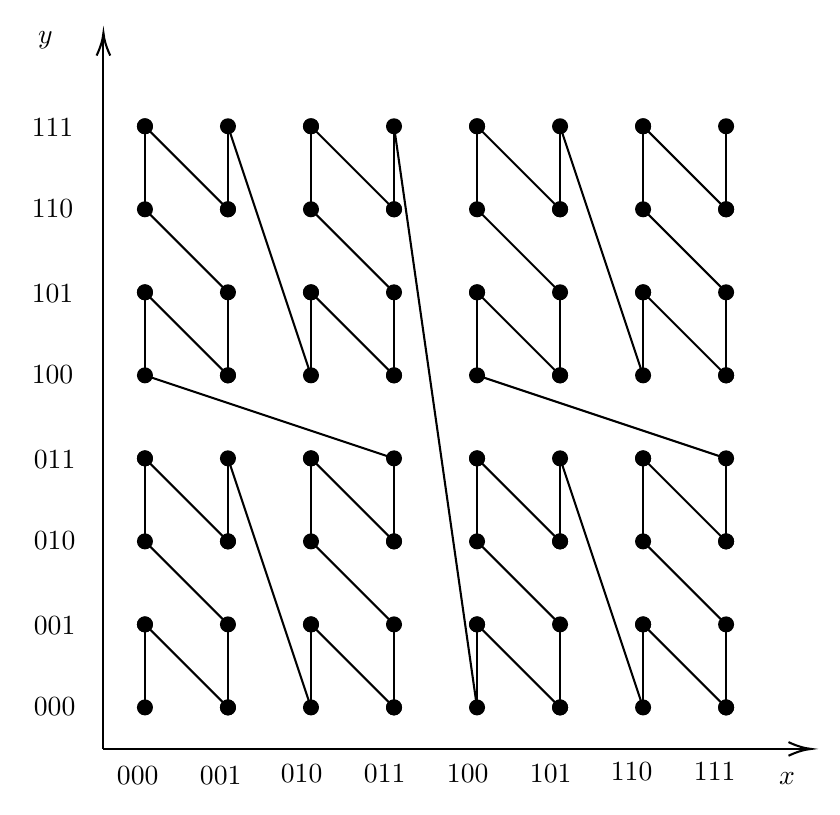
\begin{tikzpicture}[x=0.75pt,y=0.75pt,yscale=-1,xscale=1]
%uncomment if require: \path (0,498); %set diagram left start at 0, and has height of 498

%Straight Lines [id:da973386558929473] 
\draw    (50,440) -- (389,440) ;
\draw [shift={(391,440)}, rotate = 180] [color={rgb, 255:red, 0; green, 0; blue, 0 }  ][line width=0.75]    (10.93,-3.29) .. controls (6.95,-1.4) and (3.31,-0.3) .. (0,0) .. controls (3.31,0.3) and (6.95,1.4) .. (10.93,3.29)   ;
%Straight Lines [id:da21953295597080502] 
\draw    (50,440) -- (50,97) ;
\draw [shift={(50,95)}, rotate = 450] [color={rgb, 255:red, 0; green, 0; blue, 0 }  ][line width=0.75]    (10.93,-3.29) .. controls (6.95,-1.4) and (3.31,-0.3) .. (0,0) .. controls (3.31,0.3) and (6.95,1.4) .. (10.93,3.29)   ;
%Straight Lines [id:da8215679526041717] 
\draw    (70,420) -- (70,380) ;
\draw [shift={(70,380)}, rotate = 270] [color={rgb, 255:red, 0; green, 0; blue, 0 }  ][fill={rgb, 255:red, 0; green, 0; blue, 0 }  ][line width=0.75]      (0, 0) circle [x radius= 3.35, y radius= 3.35]   ;
\draw [shift={(70,420)}, rotate = 270] [color={rgb, 255:red, 0; green, 0; blue, 0 }  ][fill={rgb, 255:red, 0; green, 0; blue, 0 }  ][line width=0.75]      (0, 0) circle [x radius= 3.35, y radius= 3.35]   ;
%Straight Lines [id:da6245790210992663] 
\draw    (110,420) -- (70,380) ;
\draw [shift={(70,380)}, rotate = 225] [color={rgb, 255:red, 0; green, 0; blue, 0 }  ][fill={rgb, 255:red, 0; green, 0; blue, 0 }  ][line width=0.75]      (0, 0) circle [x radius= 3.35, y radius= 3.35]   ;
\draw [shift={(110,420)}, rotate = 225] [color={rgb, 255:red, 0; green, 0; blue, 0 }  ][fill={rgb, 255:red, 0; green, 0; blue, 0 }  ][line width=0.75]      (0, 0) circle [x radius= 3.35, y radius= 3.35]   ;
%Straight Lines [id:da12358845802318918] 
\draw    (110,420) -- (110,380) ;
\draw [shift={(110,380)}, rotate = 270] [color={rgb, 255:red, 0; green, 0; blue, 0 }  ][fill={rgb, 255:red, 0; green, 0; blue, 0 }  ][line width=0.75]      (0, 0) circle [x radius= 3.35, y radius= 3.35]   ;
\draw [shift={(110,420)}, rotate = 270] [color={rgb, 255:red, 0; green, 0; blue, 0 }  ][fill={rgb, 255:red, 0; green, 0; blue, 0 }  ][line width=0.75]      (0, 0) circle [x radius= 3.35, y radius= 3.35]   ;
%Straight Lines [id:da3864696320061456] 
\draw    (70,340) -- (70,300) ;
\draw [shift={(70,300)}, rotate = 270] [color={rgb, 255:red, 0; green, 0; blue, 0 }  ][fill={rgb, 255:red, 0; green, 0; blue, 0 }  ][line width=0.75]      (0, 0) circle [x radius= 3.35, y radius= 3.35]   ;
\draw [shift={(70,340)}, rotate = 270] [color={rgb, 255:red, 0; green, 0; blue, 0 }  ][fill={rgb, 255:red, 0; green, 0; blue, 0 }  ][line width=0.75]      (0, 0) circle [x radius= 3.35, y radius= 3.35]   ;
%Straight Lines [id:da3749246838381308] 
\draw    (110,340) -- (70,300) ;
\draw [shift={(70,300)}, rotate = 225] [color={rgb, 255:red, 0; green, 0; blue, 0 }  ][fill={rgb, 255:red, 0; green, 0; blue, 0 }  ][line width=0.75]      (0, 0) circle [x radius= 3.35, y radius= 3.35]   ;
\draw [shift={(110,340)}, rotate = 225] [color={rgb, 255:red, 0; green, 0; blue, 0 }  ][fill={rgb, 255:red, 0; green, 0; blue, 0 }  ][line width=0.75]      (0, 0) circle [x radius= 3.35, y radius= 3.35]   ;
%Straight Lines [id:da38699011412502826] 
\draw    (110,340) -- (110,300) ;
\draw [shift={(110,300)}, rotate = 270] [color={rgb, 255:red, 0; green, 0; blue, 0 }  ][fill={rgb, 255:red, 0; green, 0; blue, 0 }  ][line width=0.75]      (0, 0) circle [x radius= 3.35, y radius= 3.35]   ;
\draw [shift={(110,340)}, rotate = 270] [color={rgb, 255:red, 0; green, 0; blue, 0 }  ][fill={rgb, 255:red, 0; green, 0; blue, 0 }  ][line width=0.75]      (0, 0) circle [x radius= 3.35, y radius= 3.35]   ;
%Straight Lines [id:da09365698439534964] 
\draw    (150,420) -- (150,380) ;
\draw [shift={(150,380)}, rotate = 270] [color={rgb, 255:red, 0; green, 0; blue, 0 }  ][fill={rgb, 255:red, 0; green, 0; blue, 0 }  ][line width=0.75]      (0, 0) circle [x radius= 3.35, y radius= 3.35]   ;
\draw [shift={(150,420)}, rotate = 270] [color={rgb, 255:red, 0; green, 0; blue, 0 }  ][fill={rgb, 255:red, 0; green, 0; blue, 0 }  ][line width=0.75]      (0, 0) circle [x radius= 3.35, y radius= 3.35]   ;
%Straight Lines [id:da6092223106630459] 
\draw    (190,420) -- (150,380) ;
\draw [shift={(150,380)}, rotate = 225] [color={rgb, 255:red, 0; green, 0; blue, 0 }  ][fill={rgb, 255:red, 0; green, 0; blue, 0 }  ][line width=0.75]      (0, 0) circle [x radius= 3.35, y radius= 3.35]   ;
\draw [shift={(190,420)}, rotate = 225] [color={rgb, 255:red, 0; green, 0; blue, 0 }  ][fill={rgb, 255:red, 0; green, 0; blue, 0 }  ][line width=0.75]      (0, 0) circle [x radius= 3.35, y radius= 3.35]   ;
%Straight Lines [id:da22880765359056765] 
\draw    (190,420) -- (190,380) ;
\draw [shift={(190,380)}, rotate = 270] [color={rgb, 255:red, 0; green, 0; blue, 0 }  ][fill={rgb, 255:red, 0; green, 0; blue, 0 }  ][line width=0.75]      (0, 0) circle [x radius= 3.35, y radius= 3.35]   ;
\draw [shift={(190,420)}, rotate = 270] [color={rgb, 255:red, 0; green, 0; blue, 0 }  ][fill={rgb, 255:red, 0; green, 0; blue, 0 }  ][line width=0.75]      (0, 0) circle [x radius= 3.35, y radius= 3.35]   ;
%Straight Lines [id:da7826915277272894] 
\draw    (150,340) -- (150,300) ;
\draw [shift={(150,300)}, rotate = 270] [color={rgb, 255:red, 0; green, 0; blue, 0 }  ][fill={rgb, 255:red, 0; green, 0; blue, 0 }  ][line width=0.75]      (0, 0) circle [x radius= 3.35, y radius= 3.35]   ;
\draw [shift={(150,340)}, rotate = 270] [color={rgb, 255:red, 0; green, 0; blue, 0 }  ][fill={rgb, 255:red, 0; green, 0; blue, 0 }  ][line width=0.75]      (0, 0) circle [x radius= 3.35, y radius= 3.35]   ;
%Straight Lines [id:da9299906626674557] 
\draw    (190,340) -- (150,300) ;
\draw [shift={(150,300)}, rotate = 225] [color={rgb, 255:red, 0; green, 0; blue, 0 }  ][fill={rgb, 255:red, 0; green, 0; blue, 0 }  ][line width=0.75]      (0, 0) circle [x radius= 3.35, y radius= 3.35]   ;
\draw [shift={(190,340)}, rotate = 225] [color={rgb, 255:red, 0; green, 0; blue, 0 }  ][fill={rgb, 255:red, 0; green, 0; blue, 0 }  ][line width=0.75]      (0, 0) circle [x radius= 3.35, y radius= 3.35]   ;
%Straight Lines [id:da13509333359399966] 
\draw    (190,340) -- (190,300) ;
\draw [shift={(190,300)}, rotate = 270] [color={rgb, 255:red, 0; green, 0; blue, 0 }  ][fill={rgb, 255:red, 0; green, 0; blue, 0 }  ][line width=0.75]      (0, 0) circle [x radius= 3.35, y radius= 3.35]   ;
\draw [shift={(190,340)}, rotate = 270] [color={rgb, 255:red, 0; green, 0; blue, 0 }  ][fill={rgb, 255:red, 0; green, 0; blue, 0 }  ][line width=0.75]      (0, 0) circle [x radius= 3.35, y radius= 3.35]   ;
%Straight Lines [id:da9527545670041659] 
\draw    (70,340) -- (110,380) ;
%Straight Lines [id:da3228639642622384] 
\draw    (110,300) -- (150,420) ;
%Straight Lines [id:da8268758724925029] 
\draw    (190,380) -- (150,340) ;
%Straight Lines [id:da3182632677817132] 
\draw    (70,260) -- (70,220) ;
\draw [shift={(70,220)}, rotate = 270] [color={rgb, 255:red, 0; green, 0; blue, 0 }  ][fill={rgb, 255:red, 0; green, 0; blue, 0 }  ][line width=0.75]      (0, 0) circle [x radius= 3.35, y radius= 3.35]   ;
\draw [shift={(70,260)}, rotate = 270] [color={rgb, 255:red, 0; green, 0; blue, 0 }  ][fill={rgb, 255:red, 0; green, 0; blue, 0 }  ][line width=0.75]      (0, 0) circle [x radius= 3.35, y radius= 3.35]   ;
%Straight Lines [id:da6423355345724657] 
\draw    (110,260) -- (70,220) ;
\draw [shift={(70,220)}, rotate = 225] [color={rgb, 255:red, 0; green, 0; blue, 0 }  ][fill={rgb, 255:red, 0; green, 0; blue, 0 }  ][line width=0.75]      (0, 0) circle [x radius= 3.35, y radius= 3.35]   ;
\draw [shift={(110,260)}, rotate = 225] [color={rgb, 255:red, 0; green, 0; blue, 0 }  ][fill={rgb, 255:red, 0; green, 0; blue, 0 }  ][line width=0.75]      (0, 0) circle [x radius= 3.35, y radius= 3.35]   ;
%Straight Lines [id:da7786780830331377] 
\draw    (110,260) -- (110,220) ;
\draw [shift={(110,220)}, rotate = 270] [color={rgb, 255:red, 0; green, 0; blue, 0 }  ][fill={rgb, 255:red, 0; green, 0; blue, 0 }  ][line width=0.75]      (0, 0) circle [x radius= 3.35, y radius= 3.35]   ;
\draw [shift={(110,260)}, rotate = 270] [color={rgb, 255:red, 0; green, 0; blue, 0 }  ][fill={rgb, 255:red, 0; green, 0; blue, 0 }  ][line width=0.75]      (0, 0) circle [x radius= 3.35, y radius= 3.35]   ;
%Straight Lines [id:da4553178658987911] 
\draw    (70,180) -- (70,140) ;
\draw [shift={(70,140)}, rotate = 270] [color={rgb, 255:red, 0; green, 0; blue, 0 }  ][fill={rgb, 255:red, 0; green, 0; blue, 0 }  ][line width=0.75]      (0, 0) circle [x radius= 3.35, y radius= 3.35]   ;
\draw [shift={(70,180)}, rotate = 270] [color={rgb, 255:red, 0; green, 0; blue, 0 }  ][fill={rgb, 255:red, 0; green, 0; blue, 0 }  ][line width=0.75]      (0, 0) circle [x radius= 3.35, y radius= 3.35]   ;
%Straight Lines [id:da028923714881037288] 
\draw    (110,180) -- (70,140) ;
\draw [shift={(70,140)}, rotate = 225] [color={rgb, 255:red, 0; green, 0; blue, 0 }  ][fill={rgb, 255:red, 0; green, 0; blue, 0 }  ][line width=0.75]      (0, 0) circle [x radius= 3.35, y radius= 3.35]   ;
\draw [shift={(110,180)}, rotate = 225] [color={rgb, 255:red, 0; green, 0; blue, 0 }  ][fill={rgb, 255:red, 0; green, 0; blue, 0 }  ][line width=0.75]      (0, 0) circle [x radius= 3.35, y radius= 3.35]   ;
%Straight Lines [id:da49316216159767134] 
\draw    (110,180) -- (110,140) ;
\draw [shift={(110,140)}, rotate = 270] [color={rgb, 255:red, 0; green, 0; blue, 0 }  ][fill={rgb, 255:red, 0; green, 0; blue, 0 }  ][line width=0.75]      (0, 0) circle [x radius= 3.35, y radius= 3.35]   ;
\draw [shift={(110,180)}, rotate = 270] [color={rgb, 255:red, 0; green, 0; blue, 0 }  ][fill={rgb, 255:red, 0; green, 0; blue, 0 }  ][line width=0.75]      (0, 0) circle [x radius= 3.35, y radius= 3.35]   ;
%Straight Lines [id:da5437914069875527] 
\draw    (150,260) -- (150,220) ;
\draw [shift={(150,220)}, rotate = 270] [color={rgb, 255:red, 0; green, 0; blue, 0 }  ][fill={rgb, 255:red, 0; green, 0; blue, 0 }  ][line width=0.75]      (0, 0) circle [x radius= 3.35, y radius= 3.35]   ;
\draw [shift={(150,260)}, rotate = 270] [color={rgb, 255:red, 0; green, 0; blue, 0 }  ][fill={rgb, 255:red, 0; green, 0; blue, 0 }  ][line width=0.75]      (0, 0) circle [x radius= 3.35, y radius= 3.35]   ;
%Straight Lines [id:da570083784396854] 
\draw    (190,260) -- (150,220) ;
\draw [shift={(150,220)}, rotate = 225] [color={rgb, 255:red, 0; green, 0; blue, 0 }  ][fill={rgb, 255:red, 0; green, 0; blue, 0 }  ][line width=0.75]      (0, 0) circle [x radius= 3.35, y radius= 3.35]   ;
\draw [shift={(190,260)}, rotate = 225] [color={rgb, 255:red, 0; green, 0; blue, 0 }  ][fill={rgb, 255:red, 0; green, 0; blue, 0 }  ][line width=0.75]      (0, 0) circle [x radius= 3.35, y radius= 3.35]   ;
%Straight Lines [id:da7421199862136882] 
\draw    (190,260) -- (190,220) ;
\draw [shift={(190,220)}, rotate = 270] [color={rgb, 255:red, 0; green, 0; blue, 0 }  ][fill={rgb, 255:red, 0; green, 0; blue, 0 }  ][line width=0.75]      (0, 0) circle [x radius= 3.35, y radius= 3.35]   ;
\draw [shift={(190,260)}, rotate = 270] [color={rgb, 255:red, 0; green, 0; blue, 0 }  ][fill={rgb, 255:red, 0; green, 0; blue, 0 }  ][line width=0.75]      (0, 0) circle [x radius= 3.35, y radius= 3.35]   ;
%Straight Lines [id:da13485491953791273] 
\draw    (150,180) -- (150,140) ;
\draw [shift={(150,140)}, rotate = 270] [color={rgb, 255:red, 0; green, 0; blue, 0 }  ][fill={rgb, 255:red, 0; green, 0; blue, 0 }  ][line width=0.75]      (0, 0) circle [x radius= 3.35, y radius= 3.35]   ;
\draw [shift={(150,180)}, rotate = 270] [color={rgb, 255:red, 0; green, 0; blue, 0 }  ][fill={rgb, 255:red, 0; green, 0; blue, 0 }  ][line width=0.75]      (0, 0) circle [x radius= 3.35, y radius= 3.35]   ;
%Straight Lines [id:da6191356186785333] 
\draw    (190,180) -- (150,140) ;
\draw [shift={(150,140)}, rotate = 225] [color={rgb, 255:red, 0; green, 0; blue, 0 }  ][fill={rgb, 255:red, 0; green, 0; blue, 0 }  ][line width=0.75]      (0, 0) circle [x radius= 3.35, y radius= 3.35]   ;
\draw [shift={(190,180)}, rotate = 225] [color={rgb, 255:red, 0; green, 0; blue, 0 }  ][fill={rgb, 255:red, 0; green, 0; blue, 0 }  ][line width=0.75]      (0, 0) circle [x radius= 3.35, y radius= 3.35]   ;
%Straight Lines [id:da7672705513821019] 
\draw    (190,180) -- (190,140) ;
\draw [shift={(190,140)}, rotate = 270] [color={rgb, 255:red, 0; green, 0; blue, 0 }  ][fill={rgb, 255:red, 0; green, 0; blue, 0 }  ][line width=0.75]      (0, 0) circle [x radius= 3.35, y radius= 3.35]   ;
\draw [shift={(190,180)}, rotate = 270] [color={rgb, 255:red, 0; green, 0; blue, 0 }  ][fill={rgb, 255:red, 0; green, 0; blue, 0 }  ][line width=0.75]      (0, 0) circle [x radius= 3.35, y radius= 3.35]   ;
%Straight Lines [id:da7671970864388922] 
\draw    (70,180) -- (110,220) ;
%Straight Lines [id:da9072557577405369] 
\draw    (110,140) -- (150,260) ;
%Straight Lines [id:da5531079330221722] 
\draw    (190,220) -- (150,180) ;
%Straight Lines [id:da32751843164446615] 
\draw    (70,260) -- (190,300) ;
%Straight Lines [id:da9753894956964277] 
\draw    (230,420) -- (230,380) ;
\draw [shift={(230,380)}, rotate = 270] [color={rgb, 255:red, 0; green, 0; blue, 0 }  ][fill={rgb, 255:red, 0; green, 0; blue, 0 }  ][line width=0.75]      (0, 0) circle [x radius= 3.35, y radius= 3.35]   ;
\draw [shift={(230,420)}, rotate = 270] [color={rgb, 255:red, 0; green, 0; blue, 0 }  ][fill={rgb, 255:red, 0; green, 0; blue, 0 }  ][line width=0.75]      (0, 0) circle [x radius= 3.35, y radius= 3.35]   ;
%Straight Lines [id:da24338996217485898] 
\draw    (270,420) -- (230,380) ;
\draw [shift={(230,380)}, rotate = 225] [color={rgb, 255:red, 0; green, 0; blue, 0 }  ][fill={rgb, 255:red, 0; green, 0; blue, 0 }  ][line width=0.75]      (0, 0) circle [x radius= 3.35, y radius= 3.35]   ;
\draw [shift={(270,420)}, rotate = 225] [color={rgb, 255:red, 0; green, 0; blue, 0 }  ][fill={rgb, 255:red, 0; green, 0; blue, 0 }  ][line width=0.75]      (0, 0) circle [x radius= 3.35, y radius= 3.35]   ;
%Straight Lines [id:da6368022435216754] 
\draw    (270,420) -- (270,380) ;
\draw [shift={(270,380)}, rotate = 270] [color={rgb, 255:red, 0; green, 0; blue, 0 }  ][fill={rgb, 255:red, 0; green, 0; blue, 0 }  ][line width=0.75]      (0, 0) circle [x radius= 3.35, y radius= 3.35]   ;
\draw [shift={(270,420)}, rotate = 270] [color={rgb, 255:red, 0; green, 0; blue, 0 }  ][fill={rgb, 255:red, 0; green, 0; blue, 0 }  ][line width=0.75]      (0, 0) circle [x radius= 3.35, y radius= 3.35]   ;
%Straight Lines [id:da10669833706093867] 
\draw    (230,340) -- (230,300) ;
\draw [shift={(230,300)}, rotate = 270] [color={rgb, 255:red, 0; green, 0; blue, 0 }  ][fill={rgb, 255:red, 0; green, 0; blue, 0 }  ][line width=0.75]      (0, 0) circle [x radius= 3.35, y radius= 3.35]   ;
\draw [shift={(230,340)}, rotate = 270] [color={rgb, 255:red, 0; green, 0; blue, 0 }  ][fill={rgb, 255:red, 0; green, 0; blue, 0 }  ][line width=0.75]      (0, 0) circle [x radius= 3.35, y radius= 3.35]   ;
%Straight Lines [id:da23950201506830293] 
\draw    (270,340) -- (230,300) ;
\draw [shift={(230,300)}, rotate = 225] [color={rgb, 255:red, 0; green, 0; blue, 0 }  ][fill={rgb, 255:red, 0; green, 0; blue, 0 }  ][line width=0.75]      (0, 0) circle [x radius= 3.35, y radius= 3.35]   ;
\draw [shift={(270,340)}, rotate = 225] [color={rgb, 255:red, 0; green, 0; blue, 0 }  ][fill={rgb, 255:red, 0; green, 0; blue, 0 }  ][line width=0.75]      (0, 0) circle [x radius= 3.35, y radius= 3.35]   ;
%Straight Lines [id:da7234513308878561] 
\draw    (270,340) -- (270,300) ;
\draw [shift={(270,300)}, rotate = 270] [color={rgb, 255:red, 0; green, 0; blue, 0 }  ][fill={rgb, 255:red, 0; green, 0; blue, 0 }  ][line width=0.75]      (0, 0) circle [x radius= 3.35, y radius= 3.35]   ;
\draw [shift={(270,340)}, rotate = 270] [color={rgb, 255:red, 0; green, 0; blue, 0 }  ][fill={rgb, 255:red, 0; green, 0; blue, 0 }  ][line width=0.75]      (0, 0) circle [x radius= 3.35, y radius= 3.35]   ;
%Straight Lines [id:da2877806191384429] 
\draw    (310,420) -- (310,380) ;
\draw [shift={(310,380)}, rotate = 270] [color={rgb, 255:red, 0; green, 0; blue, 0 }  ][fill={rgb, 255:red, 0; green, 0; blue, 0 }  ][line width=0.75]      (0, 0) circle [x radius= 3.35, y radius= 3.35]   ;
\draw [shift={(310,420)}, rotate = 270] [color={rgb, 255:red, 0; green, 0; blue, 0 }  ][fill={rgb, 255:red, 0; green, 0; blue, 0 }  ][line width=0.75]      (0, 0) circle [x radius= 3.35, y radius= 3.35]   ;
%Straight Lines [id:da6137413296414147] 
\draw    (350,420) -- (310,380) ;
\draw [shift={(310,380)}, rotate = 225] [color={rgb, 255:red, 0; green, 0; blue, 0 }  ][fill={rgb, 255:red, 0; green, 0; blue, 0 }  ][line width=0.75]      (0, 0) circle [x radius= 3.35, y radius= 3.35]   ;
\draw [shift={(350,420)}, rotate = 225] [color={rgb, 255:red, 0; green, 0; blue, 0 }  ][fill={rgb, 255:red, 0; green, 0; blue, 0 }  ][line width=0.75]      (0, 0) circle [x radius= 3.35, y radius= 3.35]   ;
%Straight Lines [id:da31066746786079613] 
\draw    (350,420) -- (350,380) ;
\draw [shift={(350,380)}, rotate = 270] [color={rgb, 255:red, 0; green, 0; blue, 0 }  ][fill={rgb, 255:red, 0; green, 0; blue, 0 }  ][line width=0.75]      (0, 0) circle [x radius= 3.35, y radius= 3.35]   ;
\draw [shift={(350,420)}, rotate = 270] [color={rgb, 255:red, 0; green, 0; blue, 0 }  ][fill={rgb, 255:red, 0; green, 0; blue, 0 }  ][line width=0.75]      (0, 0) circle [x radius= 3.35, y radius= 3.35]   ;
%Straight Lines [id:da6504339520388267] 
\draw    (310,340) -- (310,300) ;
\draw [shift={(310,300)}, rotate = 270] [color={rgb, 255:red, 0; green, 0; blue, 0 }  ][fill={rgb, 255:red, 0; green, 0; blue, 0 }  ][line width=0.75]      (0, 0) circle [x radius= 3.35, y radius= 3.35]   ;
\draw [shift={(310,340)}, rotate = 270] [color={rgb, 255:red, 0; green, 0; blue, 0 }  ][fill={rgb, 255:red, 0; green, 0; blue, 0 }  ][line width=0.75]      (0, 0) circle [x radius= 3.35, y radius= 3.35]   ;
%Straight Lines [id:da7486025498386641] 
\draw    (350,340) -- (310,300) ;
\draw [shift={(310,300)}, rotate = 225] [color={rgb, 255:red, 0; green, 0; blue, 0 }  ][fill={rgb, 255:red, 0; green, 0; blue, 0 }  ][line width=0.75]      (0, 0) circle [x radius= 3.35, y radius= 3.35]   ;
\draw [shift={(350,340)}, rotate = 225] [color={rgb, 255:red, 0; green, 0; blue, 0 }  ][fill={rgb, 255:red, 0; green, 0; blue, 0 }  ][line width=0.75]      (0, 0) circle [x radius= 3.35, y radius= 3.35]   ;
%Straight Lines [id:da21318926648588832] 
\draw    (350,340) -- (350,300) ;
\draw [shift={(350,300)}, rotate = 270] [color={rgb, 255:red, 0; green, 0; blue, 0 }  ][fill={rgb, 255:red, 0; green, 0; blue, 0 }  ][line width=0.75]      (0, 0) circle [x radius= 3.35, y radius= 3.35]   ;
\draw [shift={(350,340)}, rotate = 270] [color={rgb, 255:red, 0; green, 0; blue, 0 }  ][fill={rgb, 255:red, 0; green, 0; blue, 0 }  ][line width=0.75]      (0, 0) circle [x radius= 3.35, y radius= 3.35]   ;
%Straight Lines [id:da6716171665332675] 
\draw    (230,340) -- (270,380) ;
%Straight Lines [id:da9602205048682062] 
\draw    (270,300) -- (310,420) ;
%Straight Lines [id:da28025962109893143] 
\draw    (350,380) -- (310,340) ;
%Straight Lines [id:da674384727510599] 
\draw    (230,260) -- (230,220) ;
\draw [shift={(230,220)}, rotate = 270] [color={rgb, 255:red, 0; green, 0; blue, 0 }  ][fill={rgb, 255:red, 0; green, 0; blue, 0 }  ][line width=0.75]      (0, 0) circle [x radius= 3.35, y radius= 3.35]   ;
\draw [shift={(230,260)}, rotate = 270] [color={rgb, 255:red, 0; green, 0; blue, 0 }  ][fill={rgb, 255:red, 0; green, 0; blue, 0 }  ][line width=0.75]      (0, 0) circle [x radius= 3.35, y radius= 3.35]   ;
%Straight Lines [id:da6407263647373838] 
\draw    (270,260) -- (230,220) ;
\draw [shift={(230,220)}, rotate = 225] [color={rgb, 255:red, 0; green, 0; blue, 0 }  ][fill={rgb, 255:red, 0; green, 0; blue, 0 }  ][line width=0.75]      (0, 0) circle [x radius= 3.35, y radius= 3.35]   ;
\draw [shift={(270,260)}, rotate = 225] [color={rgb, 255:red, 0; green, 0; blue, 0 }  ][fill={rgb, 255:red, 0; green, 0; blue, 0 }  ][line width=0.75]      (0, 0) circle [x radius= 3.35, y radius= 3.35]   ;
%Straight Lines [id:da2006331961573029] 
\draw    (270,260) -- (270,220) ;
\draw [shift={(270,220)}, rotate = 270] [color={rgb, 255:red, 0; green, 0; blue, 0 }  ][fill={rgb, 255:red, 0; green, 0; blue, 0 }  ][line width=0.75]      (0, 0) circle [x radius= 3.35, y radius= 3.35]   ;
\draw [shift={(270,260)}, rotate = 270] [color={rgb, 255:red, 0; green, 0; blue, 0 }  ][fill={rgb, 255:red, 0; green, 0; blue, 0 }  ][line width=0.75]      (0, 0) circle [x radius= 3.35, y radius= 3.35]   ;
%Straight Lines [id:da870681916245984] 
\draw    (230,180) -- (230,140) ;
\draw [shift={(230,140)}, rotate = 270] [color={rgb, 255:red, 0; green, 0; blue, 0 }  ][fill={rgb, 255:red, 0; green, 0; blue, 0 }  ][line width=0.75]      (0, 0) circle [x radius= 3.35, y radius= 3.35]   ;
\draw [shift={(230,180)}, rotate = 270] [color={rgb, 255:red, 0; green, 0; blue, 0 }  ][fill={rgb, 255:red, 0; green, 0; blue, 0 }  ][line width=0.75]      (0, 0) circle [x radius= 3.35, y radius= 3.35]   ;
%Straight Lines [id:da5150272168122343] 
\draw    (270,180) -- (230,140) ;
\draw [shift={(230,140)}, rotate = 225] [color={rgb, 255:red, 0; green, 0; blue, 0 }  ][fill={rgb, 255:red, 0; green, 0; blue, 0 }  ][line width=0.75]      (0, 0) circle [x radius= 3.35, y radius= 3.35]   ;
\draw [shift={(270,180)}, rotate = 225] [color={rgb, 255:red, 0; green, 0; blue, 0 }  ][fill={rgb, 255:red, 0; green, 0; blue, 0 }  ][line width=0.75]      (0, 0) circle [x radius= 3.35, y radius= 3.35]   ;
%Straight Lines [id:da729447591818692] 
\draw    (270,180) -- (270,140) ;
\draw [shift={(270,140)}, rotate = 270] [color={rgb, 255:red, 0; green, 0; blue, 0 }  ][fill={rgb, 255:red, 0; green, 0; blue, 0 }  ][line width=0.75]      (0, 0) circle [x radius= 3.35, y radius= 3.35]   ;
\draw [shift={(270,180)}, rotate = 270] [color={rgb, 255:red, 0; green, 0; blue, 0 }  ][fill={rgb, 255:red, 0; green, 0; blue, 0 }  ][line width=0.75]      (0, 0) circle [x radius= 3.35, y radius= 3.35]   ;
%Straight Lines [id:da7687667597351182] 
\draw    (310,260) -- (310,220) ;
\draw [shift={(310,220)}, rotate = 270] [color={rgb, 255:red, 0; green, 0; blue, 0 }  ][fill={rgb, 255:red, 0; green, 0; blue, 0 }  ][line width=0.75]      (0, 0) circle [x radius= 3.35, y radius= 3.35]   ;
\draw [shift={(310,260)}, rotate = 270] [color={rgb, 255:red, 0; green, 0; blue, 0 }  ][fill={rgb, 255:red, 0; green, 0; blue, 0 }  ][line width=0.75]      (0, 0) circle [x radius= 3.35, y radius= 3.35]   ;
%Straight Lines [id:da7294378004965458] 
\draw    (350,260) -- (310,220) ;
\draw [shift={(310,220)}, rotate = 225] [color={rgb, 255:red, 0; green, 0; blue, 0 }  ][fill={rgb, 255:red, 0; green, 0; blue, 0 }  ][line width=0.75]      (0, 0) circle [x radius= 3.35, y radius= 3.35]   ;
\draw [shift={(350,260)}, rotate = 225] [color={rgb, 255:red, 0; green, 0; blue, 0 }  ][fill={rgb, 255:red, 0; green, 0; blue, 0 }  ][line width=0.75]      (0, 0) circle [x radius= 3.35, y radius= 3.35]   ;
%Straight Lines [id:da7617568659839697] 
\draw    (350,260) -- (350,220) ;
\draw [shift={(350,220)}, rotate = 270] [color={rgb, 255:red, 0; green, 0; blue, 0 }  ][fill={rgb, 255:red, 0; green, 0; blue, 0 }  ][line width=0.75]      (0, 0) circle [x radius= 3.35, y radius= 3.35]   ;
\draw [shift={(350,260)}, rotate = 270] [color={rgb, 255:red, 0; green, 0; blue, 0 }  ][fill={rgb, 255:red, 0; green, 0; blue, 0 }  ][line width=0.75]      (0, 0) circle [x radius= 3.35, y radius= 3.35]   ;
%Straight Lines [id:da2507214814275216] 
\draw    (310,180) -- (310,140) ;
\draw [shift={(310,140)}, rotate = 270] [color={rgb, 255:red, 0; green, 0; blue, 0 }  ][fill={rgb, 255:red, 0; green, 0; blue, 0 }  ][line width=0.75]      (0, 0) circle [x radius= 3.35, y radius= 3.35]   ;
\draw [shift={(310,180)}, rotate = 270] [color={rgb, 255:red, 0; green, 0; blue, 0 }  ][fill={rgb, 255:red, 0; green, 0; blue, 0 }  ][line width=0.75]      (0, 0) circle [x radius= 3.35, y radius= 3.35]   ;
%Straight Lines [id:da5857592927516508] 
\draw    (350,180) -- (310,140) ;
\draw [shift={(310,140)}, rotate = 225] [color={rgb, 255:red, 0; green, 0; blue, 0 }  ][fill={rgb, 255:red, 0; green, 0; blue, 0 }  ][line width=0.75]      (0, 0) circle [x radius= 3.35, y radius= 3.35]   ;
\draw [shift={(350,180)}, rotate = 225] [color={rgb, 255:red, 0; green, 0; blue, 0 }  ][fill={rgb, 255:red, 0; green, 0; blue, 0 }  ][line width=0.75]      (0, 0) circle [x radius= 3.35, y radius= 3.35]   ;
%Straight Lines [id:da06335255779537685] 
\draw    (350,180) -- (350,140) ;
\draw [shift={(350,140)}, rotate = 270] [color={rgb, 255:red, 0; green, 0; blue, 0 }  ][fill={rgb, 255:red, 0; green, 0; blue, 0 }  ][line width=0.75]      (0, 0) circle [x radius= 3.35, y radius= 3.35]   ;
\draw [shift={(350,180)}, rotate = 270] [color={rgb, 255:red, 0; green, 0; blue, 0 }  ][fill={rgb, 255:red, 0; green, 0; blue, 0 }  ][line width=0.75]      (0, 0) circle [x radius= 3.35, y radius= 3.35]   ;
%Straight Lines [id:da45000361974348846] 
\draw    (230,180) -- (270,220) ;
%Straight Lines [id:da6833780770927858] 
\draw    (270,140) -- (310,260) ;
%Straight Lines [id:da6551201913810607] 
\draw    (350,220) -- (310,180) ;
%Straight Lines [id:da2428759594498866] 
\draw    (230,260) -- (350,300) ;
%Straight Lines [id:da8816068593133708] 
\draw    (190,140) -- (230,420) ;

% Text Node
\draw (374,450) node [anchor=north west][inner sep=0.75pt]   [align=left] {$\displaystyle x$};
% Text Node
\draw (17,93) node [anchor=north west][inner sep=0.75pt]   [align=left] {$\displaystyle y$};
% Text Node
\draw (55,447) node [anchor=north west][inner sep=0.75pt]   [align=left] {$\displaystyle 000$};
% Text Node
\draw (95,447) node [anchor=north west][inner sep=0.75pt]   [align=left] {$\displaystyle 001$};
% Text Node
\draw (134,446) node [anchor=north west][inner sep=0.75pt]   [align=left] {$\displaystyle 010$};
% Text Node
\draw (174,446) node [anchor=north west][inner sep=0.75pt]   [align=left] {$\displaystyle 011$};
% Text Node
\draw (214,446) node [anchor=north west][inner sep=0.75pt]   [align=left] {$\displaystyle 100$};
% Text Node
\draw (254,446) node [anchor=north west][inner sep=0.75pt]   [align=left] {$\displaystyle 101$};
% Text Node
\draw (293,445) node [anchor=north west][inner sep=0.75pt]   [align=left] {$\displaystyle 110$};
% Text Node
\draw (333,445) node [anchor=north west][inner sep=0.75pt]   [align=left] {$\displaystyle 111$};
% Text Node
\draw (15,414) node [anchor=north west][inner sep=0.75pt]   [align=left] {$\displaystyle 000$};
% Text Node
\draw (15,375) node [anchor=north west][inner sep=0.75pt]   [align=left] {$\displaystyle 001$};
% Text Node
\draw (15,334) node [anchor=north west][inner sep=0.75pt]   [align=left] {$\displaystyle 010$};
% Text Node
\draw (15,295) node [anchor=north west][inner sep=0.75pt]   [align=left] {$\displaystyle 011$};
% Text Node
\draw (14,254) node [anchor=north west][inner sep=0.75pt]   [align=left] {$\displaystyle 100$};
% Text Node
\draw (14,215) node [anchor=north west][inner sep=0.75pt]   [align=left] {$\displaystyle 101$};
% Text Node
\draw (14,174) node [anchor=north west][inner sep=0.75pt]   [align=left] {$\displaystyle 110$};
% Text Node
\draw (14,135) node [anchor=north west][inner sep=0.75pt]   [align=left] {$\displaystyle 111$};


\end{tikzpicture}

    
\end{figure}


\newpage
\thispagestyle{empty}
\enlargethispage{5\baselineskip}

The morton code has many useful properties. To begin with, the most significant bit of $M$ determines exactly whether the primitive is located in the left half or the right half the scene, and the 2nd most significant bit determines whether it is located in the upper or the lower half. Continuing this pattern, for any rectangular region of the space defined by the first $k$ significant bits, the ($k+1$)th significant bit would split that region of space into two parts, alongside one of the coordinate axises. This structure is in good correspondence with the mid-point BVH splitting strategy.


Given the morton codes of all primitives, one could straightforwardly construct a binary prefix tree where the $i$th level contains $2^i$ nodes, each of which corresponds to an assignment of the first $i$ bits of a morton code. However, such a tree would not correspond to a useful BVH. This is because geometries are always distributed \textit{sparsely} in the scenes, and thus only a very small portion of the $2^{63}$ morton code values are actually used by some geometry. Thus, the algorithm \cite{bvh_build} implemented in this project uses a variant of prefix tree known as the radix tree, which compactly stores sparsely distributed keys.

For a set of $N$ binary keys $k_0,...,k_{N-1}$, a binary radix tree is binary tree whose leaves are the keys in sorted order. Each interior node $n$ in the tree is also labeled by a bit sequence, which is the longest common prefix of all leaves in the subtree rooted at $n$. Using $\delta(i,j)$ to denote the length of the longest common prefix between $k_i$ and $k_j$, the ordering of leaves implies that if $i\leq i'\leq j'\leq j$, then $\delta(i,j)\geq \delta(i',j')$. Thus, for a node whose leftmost descendent is $k_i$ and rightmost descendent $k_j$, its prefix has length exactly $\delta(i,j)$. 


In the radix tree, each internal node partitions its keys using the first differing bit, i.e. the $\delta(i,j)$th bit counting from 0. By definition, since $\delta(i,j)$ is the maximum length of common prefix, there must exists at least two keys that defer on the $\delta(i,j)$th bit. More precisely, let $k_{\gamma}$ be the rightmost key in this subtree whose $\delta(i,j)$th bit is $0$, then $k_{\gamma+1}$ must be such that the $\delta(i,j)$th bit is $1$. The radix tree partitions this interior node so that the left child covers keys $k_i$ to $k_\gamma$, and the right child covers keys $k_{\gamma+1}$ to $k_{j}$. An example radix tree with 8 5-bit keys are shown in the figure below.
\begin{figure}[H]
    \centering
    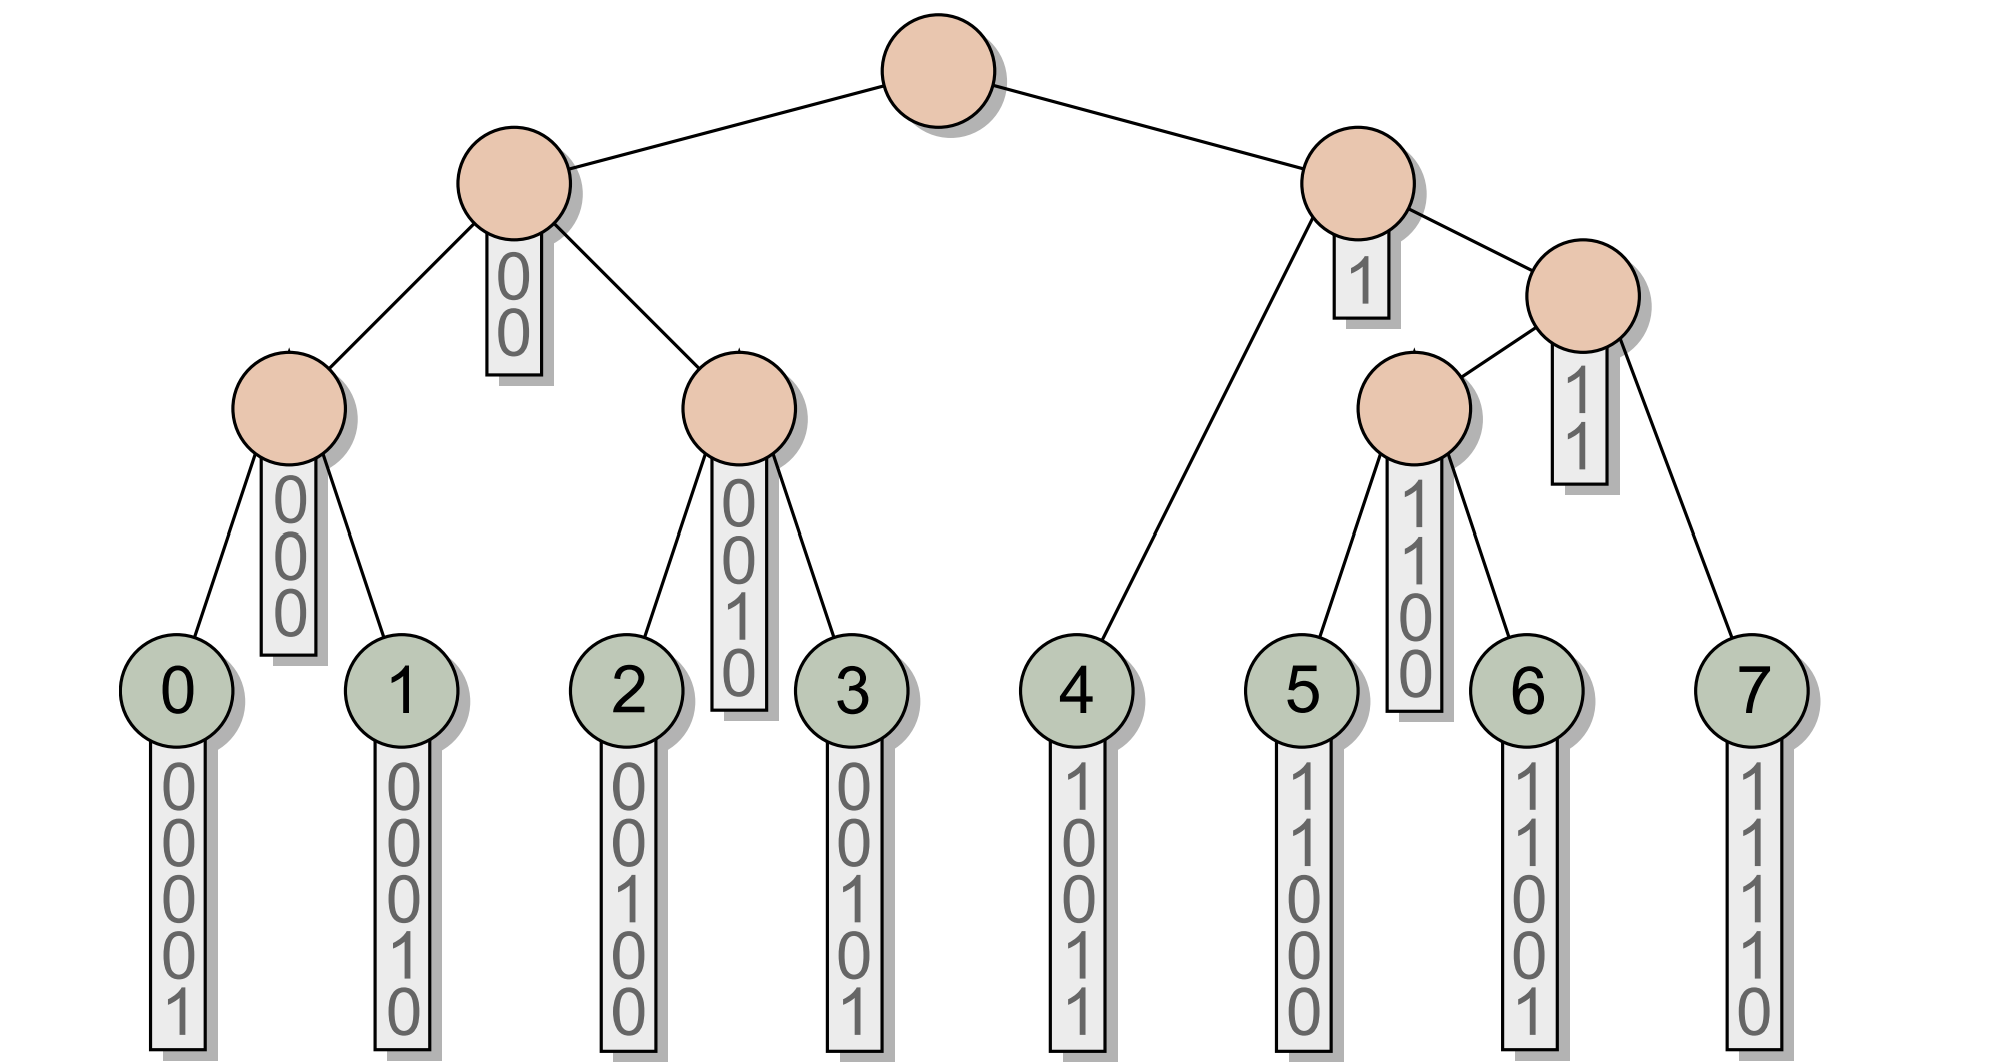
\includegraphics[height=5cm]{radix}
    \caption{Example radix tree. Image credit \cite{bvh_build}}
    \label{image radix tree}
\end{figure} 


In order to construct radix trees in parallel, the algorithm \cite{bvh_build} establishes a connection between node indices and keys through a specific tree layout, which enables any interior node to be built simultaneously with its children. The layout stores interior and leaf nodes in two separate arrays, $I$ and $L$. The leaf array is sorted on the keys increasingly, and the interior array is arranged such that
\begin{enumerate}
    \item The root of the tree is at $I_0$.
    
    \item For each interior node $n$ which covers keys $k_i,...,k_j$ and splits at $k_\gamma$: the left child is stored at $I_\gamma$ if it is also an interior node, or at $L_\gamma$ if it is a leaf. Similarly, the right child is stored at either $I_{\gamma+1}$ if it is interior, or at $L_{\gamma+1}$ if it is a leaf.
\end{enumerate}

Notice that, these two rules enforce a special property: the index of an interior node coincides with the index of either its leftmost leaf descendent, or its rightmost leaf descendent. This property is visualized in the following image, where each horizontal bar represents the range of keys covered by an interior node.
\begin{figure}[H]
    \centering
    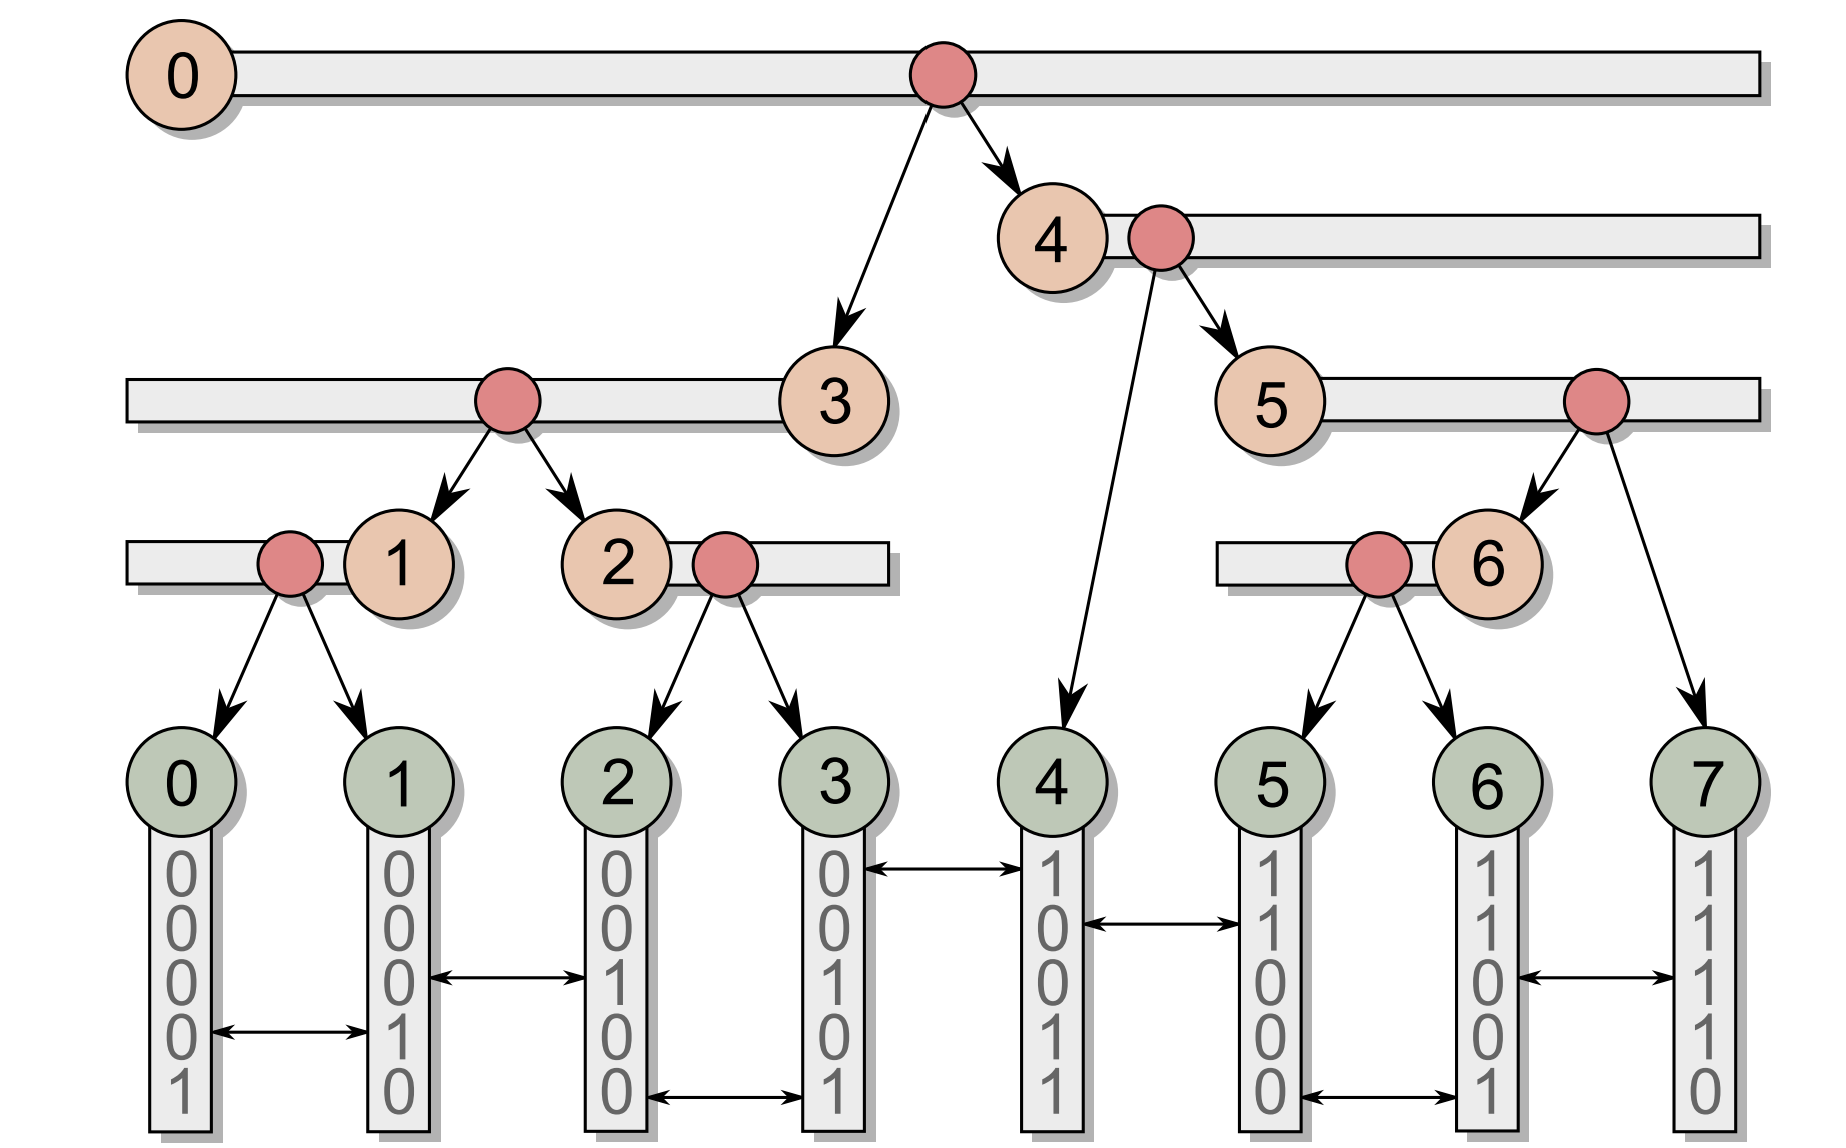
\includegraphics[height=5cm]{radix_layout.png}
    \caption{Radix tree storage layout. Image credit \cite{bvh_build}.}
\end{figure}

Given an interior node, it is not too hard to find out whether its index corresponds to the leftmost descendent, or the rightmost one. More precisely, for the interior node $I_{x}$, it suffices to compare $\delta(x,x+1)$ and $\delta(x,x-1)$. If the former is larger, then $x$ must be the index of the leftmost descendent, and otherwise $x$ coincides with the rightmost descendent. Furthermore, the smaller value of $\delta(x,x+1)$ and $\delta(x,x-1)$ provides a minimum threshold of the maximum common prefix length $\delta(i,j)$ for $I_x$, that is, $\delta(i,j)> \text{min}(\delta(x,x+1),\delta(x,x-1))$. This is because, the minimum of $\delta(x,x+1)$ and $\delta(x,x-1)$ must equal the maximum common prefix length of the parent of $I_x$, and since $L_x$ is the children, it must have a greater maximum common prefix length. 

At this point, the algorithm knowns one of $i$ and $j$, and it also knows a lower-bound $\delta_{\text{min}}$ for $\delta(i,j)$. Without loss of generality, assume that the leftmost index $i$ is known. Notice that, $j$ is a value that satisfies $\delta(i,j)>\delta_{\text{min}}$, and it must be the maximum index that does so. Thus, it suffices to perform a binary search in the interval $[i+1,N]$, and find the largest $j$ that satisfies $\delta(i,j)>\delta_{\text{min}}$. 

Having computed the leftmost and rightmost descendants $i,j$ and the maximum common prefix length $\delta(i,j)$, it only remains to identify the index of the two children, $\gamma$ and $\gamma+1$. Notice that, since $\gamma$ is the rightmost index that still belongs in the left child, it is known that $\delta(i,\gamma)>\delta(i,j)$, and $\gamma$ is the largest index in $[i,j]$ that satisfies this property. Thus, it is again straightforward to use binary search to find $\gamma$. 

For each internal node $I_x$, the algorithm identifies its two children without requiring the children to have been constructed already. Thus, the algorithm can be parallelized across all nodes. The following pseudo-code summarizes this procedure:

\begin{algorithm}[H]
    \label{algo construct radix tree}
    \SetKwProg{Fn}{Function}{:}{end}
    \ForEach{\upshape internal node $L_x$ \textbf{in parallel}}{
        $\delta_{\text{min}} := \text{min}(\delta(x,x+1),\delta(x,x-1))$ \;
        \uIf{$\delta(x,x+1)>\delta(x,x-1)$}{
            $i:=x$\;
            Binary search to find the largest $j$ such that $\delta(i,j)>\delta_{\text{min}}$\;
        }
        \Else{
            $j:=x$ \;
            Binary search to find the smallest $i$ such that $\delta(i,j)>\delta_{\text{min}}$\;
        }
        Binary search to find the biggest $\gamma$ such that $\delta(i,\gamma)>\delta(i,j)$\;
        Left child is $I_{\gamma}$ as long as $i\neq \gamma$, and $L_{\gamma}$ otherwise\;
        Right child is $I_{\gamma+1}$ as long as $j\neq \gamma+1$, and $L_{\gamma+1}$ otherwise\;
        

    }
    \caption{Parallel Binary Radix Tree Construction}
\end{algorithm} 

~ 

One caveat with this algorithm is that no duplicates are allowed in the keys $k_0,...,k_{N-1}$. However, morton codes for two geometries could potentially be identical, if they're really close together. This problem can be easily taken care of by appending extra bits after the morton code and ensuring that all binary keys are distinct.

Having constructed the binary radix tree, it only remains to convert it into a BVH by computing an AABB for each node. This can be done in parallel by having all threads start at leaf nodes, move up the tree, and repeatedly compute the AABB for the current node along the way. Whenever two sibling threads move up to process a common parent, the two threads carry out a simple consensus operation to decide which thread should drop out and terminate. 

%\enlargethispage{3\baselineskip}

This project implemented this BVH construction in CUDA. Thanks to the parallel nature of this algorithm, the project observed that the running time of this BVH construction algorithm is almost negligible ($\sim$50ms for 1 million primitives) compared to the cost of the actual path-tracing phase ($\sim$10 minutes for a 1024 $spp$ render).


\subsection{BVH Optimization}
The BVH trees constructed by the algorithm from the previous section can immensely accelerate intersection detections and thus rendering. However, the quality of these trees are still quite poor compared to trees generated with the guidance of the SAH heuristic. To address this issue, this project implements the algorithm described in \cite{bvh_optimize}, which optimizes existing BVH trees. With little running time cost, this optimization step boosts the rendering efficiency by about $300\%$.

It is believed that finding the optimal tree under the SAH heuristic is NP-hard \cite{bvh_optimize}. However, intuitively, if the tree is optimal in every local \textit{treelet}, the entire tree would be somewhat optimal. Formally, a \textit{treelet} rooted at some node is defined to be a collection of immediate descendants of the root, consisting of $m-1$ internal nodes and $m$ leaf nodes (which can still be internal nodes in the complete tree). The algorithm solves the SAH optimization problem using dynamic programming for each treelet with 7 leaves, in the hope that these local transformations improve the structure of the entire tree. 

\begin{figure}[H]
    \centering
    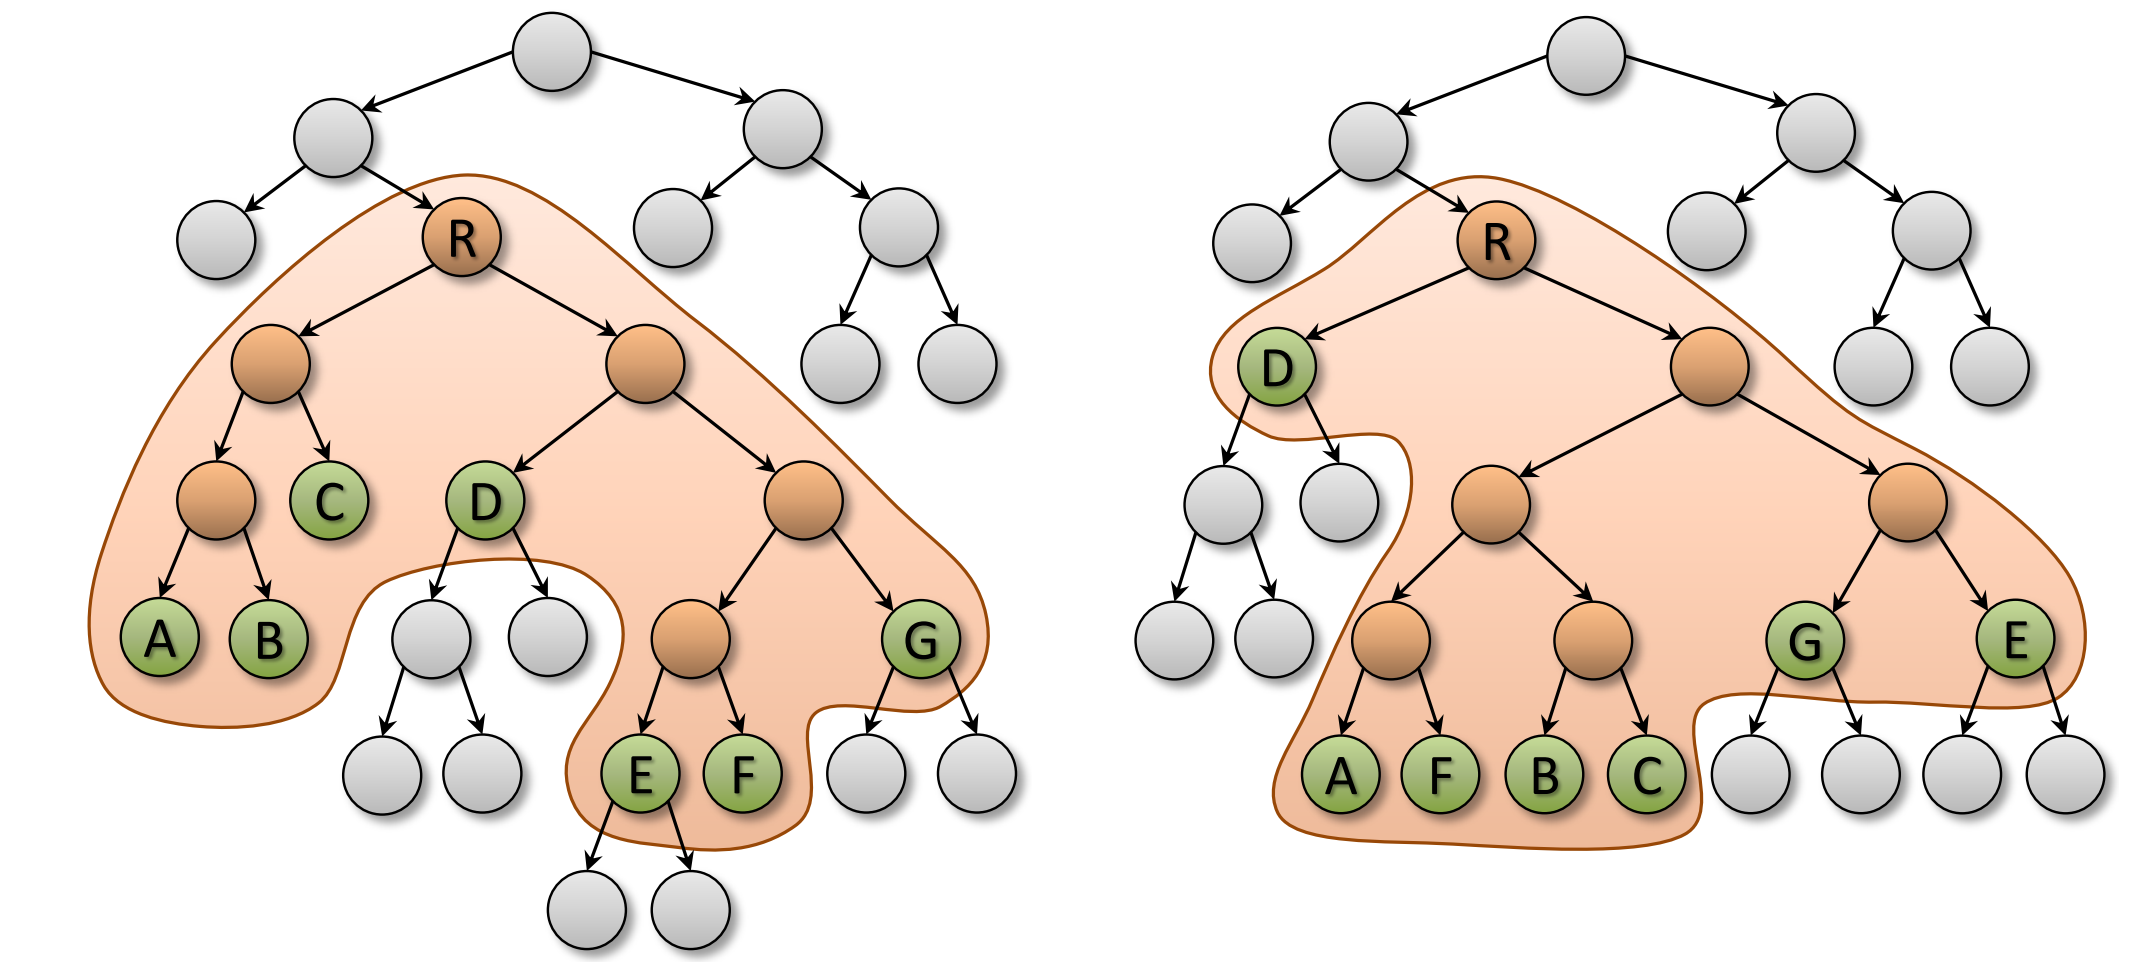
\includegraphics[height=5cm]{treelet.png}
    \caption{A treelet with 7 leaves and how it can be transformed. Image credit \cite{bvh_optimize}}
\end{figure}
For each internal node $n$, the algorithm defines its cost to be 
\begin{align*}
    C(n) = 
    \begin{cases}
        C_i A(n) + C(n_l) + C(n_r) &\text{if $n$ is an interior node in the full BVH}\\
        C_l A(n) &\text{if $n$ is a leaf node in the full BVH}\\
    \end{cases}
\end{align*}
where $n_l$ and $n_r$ are the left and right child. The cost defined this way is exactly the SAH cost multiplied by a constant factor of $A(root)$. For each internal node $n$ that is the root of a treelet with 7 leaves, the algorithm optimizes $C(n)$ by finding the optimal structure of a local treelet. If more than one treelets with 7 leaves are rooted at $n$, the algorithm operates on the one where the leaves have the greatest surface area, which maximizes the potential for improvements. 

The algorithm optimizes treelets via dynamic programing. Specifically, it optimizes subsets of leaves of increasing size, and memoizes intermediate results. When working on a size-$k$ subset $S$, it suffices to enumerate all possible binary partitions of $S$, and use memoized results to obtain optimal tree structure for each partition. Then, when the entire set of leaves is optimized, the treelet itself is also optimized. The procedure for optimizing each treelet is given in the following pseudo-code:

\begin{algorithm}[H]
    \label{algo optimize treelet}
    \SetKwProg{Fn}{Function}{:}{end}
    Create memoization array $C_{opt}$ of size $2^7$, indexed by subsets of the leaves (empirically represented as bitmaps by 7-bit integers)\;
    \ForEach{\upshape leaf node $n$ of the treelet}{
        $C_{opt}[\{n\}] := C(n)$\;
    }
    \For{\upshape $k$ from $2$ to $7$}{
        \ForEach{\upshape subset $S$ of the leaves of size $k$}{
            $C_{opt}[S] := \infty$\;
            $A(S) :=$ surface area of the AABB that encloses all primitives in $S$\;
            \ForEach{\upshape pair of disjoint nonempty subsets $U,V$, where $U\cup V=S$}{
                $thisCost := A(S)C_i + C_{opt}[U] + C_{opt}[V]$\;
                \If{\upshape $thisCost<C_{opt}[S]$}{
                    $C_{opt}[S] := thisCost$\;
                    Record $(U,V)$ as current best partition for $S$\; 
                }
            }
        }
    }
    Restructure the treelet using the best partitions found\;
    \caption{Treelet Optimization}
\end{algorithm} 

~

For treelets rooted at the same level in the BVH, this optimization step can be parallelized because the treelets do not overlap. Thus, this project implemented the algorithm in GPU, where nodes across each level are processed in parallel. Again, this step is extremely efficient, taking approximately 200ms for a scene with 1 million triangle. For such scenes rendered at 1024 $spp$, this optimization step could reduce rendering time from around 30 minutes to around 10 minutes.

\thispagestyle{empty}
\enlargethispage{5\baselineskip}

Interestingly, the optimization does not reach a fixed point after processing each treelet once. The following image plots how the SAH (and thus rendering time) changes when the BVH is optimized repeatedly. This project runs the optimization for 3 rounds for each scene, which almost always reduces SAH to $\frac{1}{3}$ of the origin value.

\begin{figure}[H]
    \centering
    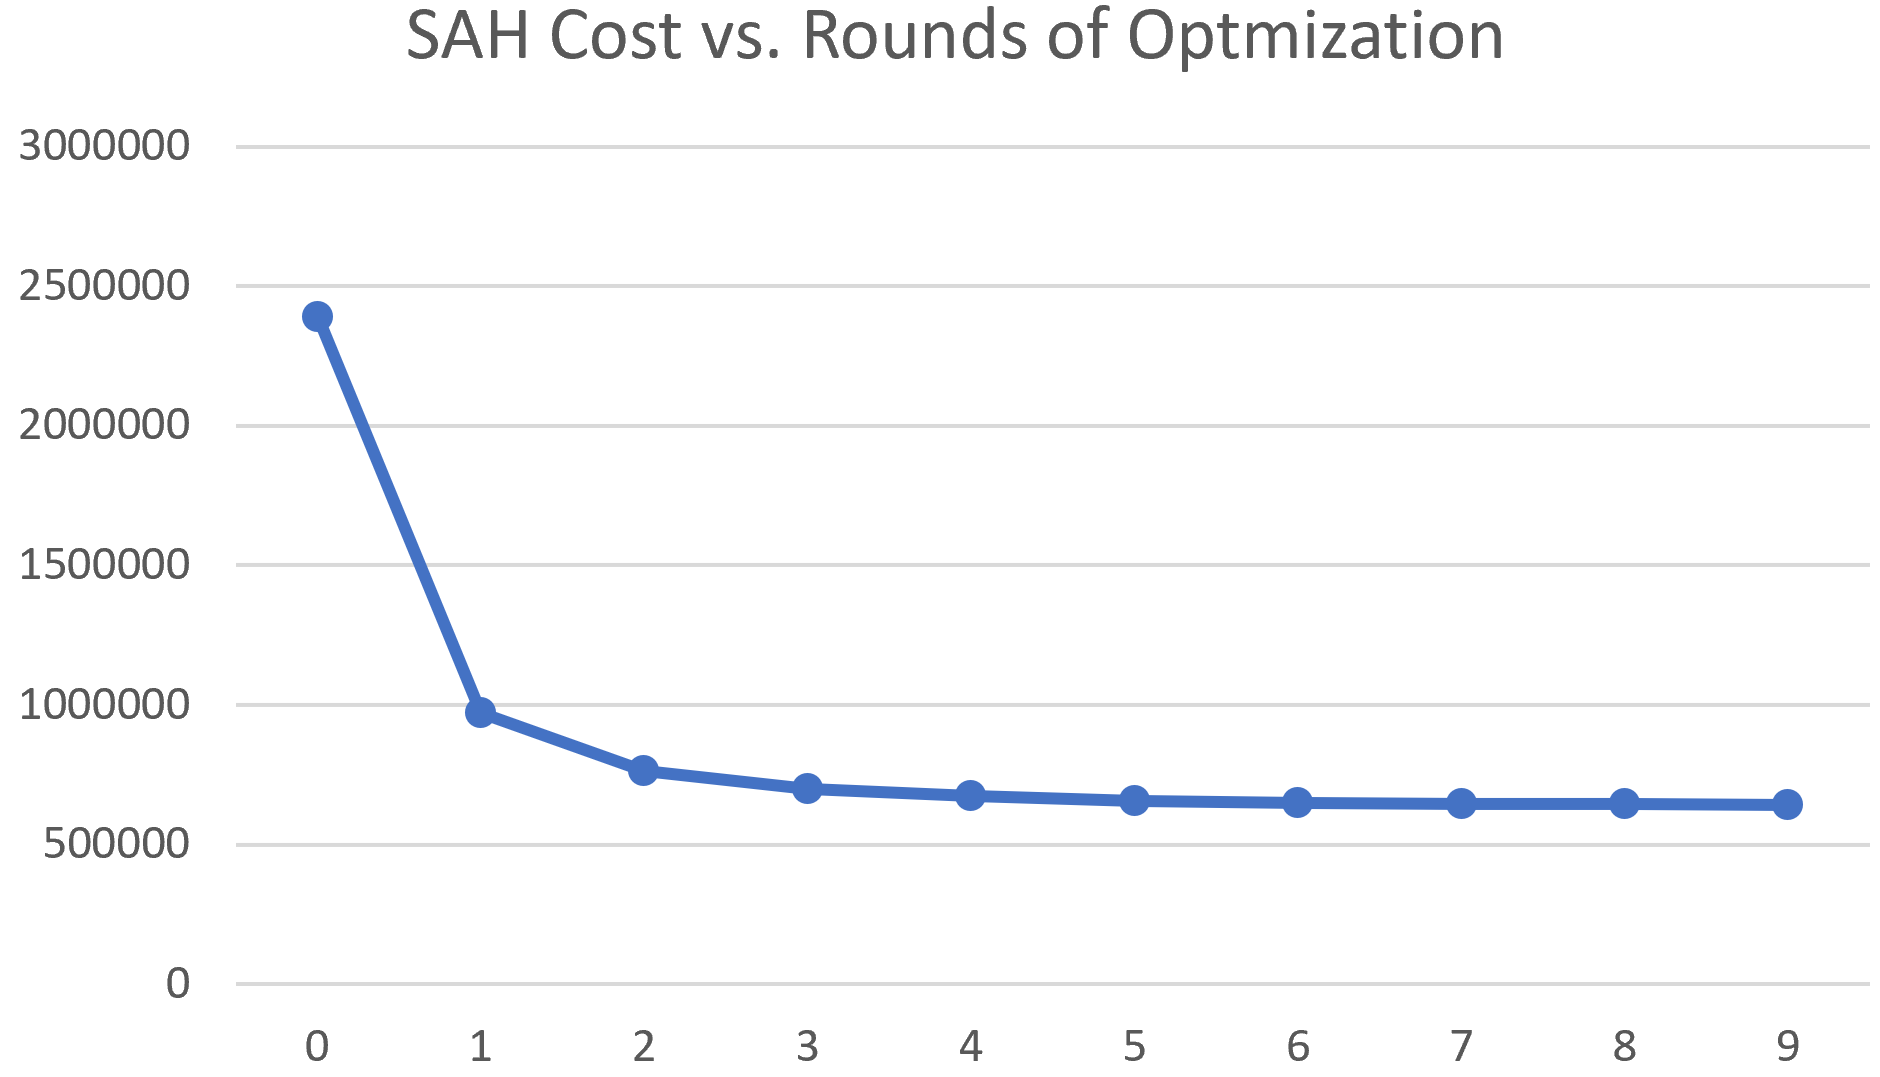
\includegraphics[height=5cm]{opt_rounds}
\end{figure}

